\section{Market-level Optimization}\label{section:market}

The original design of \Cyclus included a notion of markets that presumed a
universal objective function for ascribing a value to resources offered for a
trade.  All consumers would submit their requests and all suppliers would
declare what resources they were able to offer, and the market would apply
some algorithm to match offers with requests.  While it did provide a
capability of swapping market models, it quickly became apparent that this
solution presumes a universal function for ascribing value to individual
quanta of material, while different facilities would generally have very
different ways of assessing the relative value of different resource offers.

This section describes the capability that allows \Cyclus to match consumer
requests with supplier offers while remaining consistent with the fundamental
goals of the \Cyclus framework.  In particular, this capability must support
the following.

\vspace{1em}
\noindent\textbf{Flexibility}: In order to support a maximum level of
flexibility in \Cyclus, each agent must operate as a \textit{black box}, with
no assumed knowledge of the capabilities or current state of other agents.
This permits individual facilities to be represented by plugins that can be
swapped individually without imposing restrictions on other agents in the
system.  The market clearing mechanism must be able to accept any request for
resources, regardless of its ability to be satisfied by the system.

\vspace{1em}
\noindent\textbf{Fungibility}: Since different fissile nuclides can fill
similar roles in the fuel cycle, resource offers may differ in composition but
still satisfy the needs of the consumer.  The market clearing mechanism must
be able to accept any offer of resources, without judgement on whether or not
it meets the goals of the corresponding request.

\vspace{1em}
\noindent\textbf{Agency}: Given the prior two characteristics, the final
ability to determine the details of a specific request, a specific offer, or
which offer is the most suitable match to a specific request must rest solely
in the hands of the facilities making those requests and offers.  The market
clearing mechanism may not impose any problem-wide value judgement on the
transactions.
\vspace{1em}

A market clearing mechanism that satisfies these high level requirements,
known as the \gls{DRE}, was designed and implemented.  \ref{subsection:dre}
first discusses the conceptual design of the \gls{DRE}, followed by a formal
definition of this system as a mixed-integer linear program to solve a
modified network flow problem.  Different solvers were studied to assess the
trade-off between accuracy and efficiency.  A number of sample problems are
presented to demonstrate the capability of the \gls{DRE}.  A more
comprehensive treatment of the \gls{DRE} can be found in \citeprod{dre_paper}
and \citeprod{gidden_thesis}.  Although the \gls{DRE} provides the necessary
components for market clearing in \Cyclus, it does not lead to the most
computationally efficient results.  In particular, the \gls{DRE} does not
provide a mechanism for suppliers to tailor their offers to the specific
interests of the consumers, even if their behavior models would allow them to
do so.  \ref{subsection:callback} introduces just such a mechanism, also
allowing suppliers to ascribe differening values to different offers for use
in resolving the \gls{DRE}.

\subsection{Dynamic Resource Exchange}\label{subsection:dre}

\subsubsection{Conceptual Design}

At the conceptual level, the \gls{DRE} implements the following communication
cycle at each time step in a \Cyclus simulation:
\begin{enumerate}
\item All consumers broadcast their requests to all suppliers.  Each request
  describes the desired quantity and quality (isotopic composition).
\item Suppliers respond to each consumer request with an offer to supply
  material.  Each supplier has the agency to decide whether or not to respond,
  and if so, how to respond.  Each offer describes an available quantity and
  quality.
\item Consumers use their own valuation process to rank the offers using the
  notion of preference.
\item All preferences are collected to be solved by a system that maximizes
  the total preference in the system.
\item The solution identifies specific resource trades that are then carried
  out among the facilities/agents.
\end{enumerate}

A the heart of the \gls{DRE} is a the \gls{MTP} \citeref{even1975complexity}
which belongs to the network flow family of optimization problems. A network
flow problem is represented by a graph, $G(N, A)$, comprises nodes $N$ and
arcs $A$. If flow can occur between some node $i$ and some other node $j$,
then it flows along arc $(i, j)$. Given a graph instance, optimal flow between
nodes can be found provided \textit{objective coefficients} and
\textit{constraints}. \textit{Decision variables} for this optimization
problem comprise the optimal \textit{flow assignment}. If all decision
variables are linear, then the resulting formulation is termed a \gls{LP}. If
some decision variables are integer (e.g., binary), the formulation is termed
a \gls{MILP}.

Transportation problems model the flow of a commodity between source nodes and
sink nodes which can have supply and demand constraints. A more complex
transportation-problem formulation can support systems in which supply or demand
can be met by multiple commodities.  There is a unit cost $c_{i,j}^{h}$ for
commodity $h$ to traverse arc $(i,j)$. A supplier of commodity $h$ has a certain
supply capacity $s_i^h$ which cannot be surpassed and consumers of commodity $h$
have a certain demand level which must be met, $d_i^h$.

In the simplest extension from the single-commodity to multi-commodity
transportation problem, arc constraints for all commodities are combined,
i.e., there is a single capacity $u_{i,j}$ for a given arc $(i, j)$. A classic
application of this enhanced complexity deals with data networks. Multiple
classifications of data exist, but they all must traverse the same network
infrastructure. Accordingly, the infrastructure can only accommodate a certain
quantity of total flow among all communication types.

A number of adjustments are made to a canonical MTP to accommodate specific
features of a nuclear fuel cycle, transforming it into a so-called
\gls{NFCTP}.

\begin{enumerate}
\item 
\end{enumerate}

\subsubsection{Mathematical Formulation}


The formulation of the multi-commodity flow problem is shown in Equation
\ref{eqs:MCTP}, in which the solutions are the set of flows of each commodity
between each request-bid pair, $\{x_{i,j}^h\}$. Note the commodity
coupling in Equation \ref{eqs:MCTP_cap}.

%%% 
\begin{subequations}\label{eqs:MCTP}
  \begin{align}
    %%
    \min_{x} \:\: & 
    \sum_{i \in I}\sum_{j \in J}\sum_{h \in H} c_{i,j}^{h} x_{i,j}^{h}
    & \label{eqs:MCTP_obj} \\
    %%
    \text{s.t.} \:\: 
    &
    \sum_{i \in I} x_{i,j}^{h} \geq d_{j}^{h}
    & 
    \forall \: j \in J, \forall \: h \in H \label{eqs:MCTP_dem} \\
    %%
    &
    \sum_{j \in J} x_{i,j}^{h} \leq s_{i}^{h}
    &
    \forall \: i \in I, \forall \: h \in H \label{eqs:MCTP_sup} \\
    %%
    &
    \sum_{h \in H} x_{i,j}^{h} \leq u_{i,j}
    & 
    \forall \: (i, j) \in A \label{eqs:MCTP_cap} \\
    %%
    &
    x_{i,j}^{k} \geq 0
    &
    \forall \: (i, j) \in A, \forall \: h \in H \label{eqs:MCTP_x}
    %%
  \end{align}
\end{subequations}
%%% 


A number of specific modifications can be made to accommodate specific
features of the nuclear fuel cycle, including:
\begin{itemize}
\item portfolios of requests, $R$, and offers, $S$, that represent the
  fungibility of resources,
\item partitioning of the graph into individual commodities,
\item multiple constraints, $k \in K_{\{s,r\}}$, on indivdiual suppliers or consumers,
\item constraints that depend on the quality of the individual trade (e.g. SWU
  constraints), $a_{i,j}^k$, and
\item mutually exclusive requests, $\tilde{x_j}$, that must be fulfilled by a
  single supplier such that $x_{i,j} = \tilde{x_j} y_{i,j}$ (e.g all fuel
  assemblies should come from the same fuel fabrication facility).
\end{itemize}
This allows the \gls{MTP} to be redefined into a more problem specific
\gls{NFCTP} as shown in Equation \ref{eqs:NFCTP}.  A more detailed discussion
of these details is available in ref \citeprod{dre_paper}.

\begin{subequations}\label{eqs:NFCTP}
  \begin{align}
    %%
    \min_{x, y} \:\: 
    & 
    z \:\: = 
    \sum_{(i, j) \in A_p} c_{i,j} x_{i,j} 
    \: + 
    \sum_{(i, j) \in A_e} c^{\prime}_{i,j} y_{i,j} 
    & 
    \label{eqs:NFCTP_obj} \\
    %%
    \text{s.t.} \:\:
    &
    \sum_{(i, j) \in A_{p_r}} a^k_{i,j} x_{i,j}
    \: + 
    \sum_{(i, j) \in A_{e_r}} a^{k\prime}_{i,j} y_{i,j}
    \geq b^k_r 
    &
    \: 
    \forall \: k \in K_r,  
    \forall \: r \in R 
    \label{eqs:NFCTP_req} \\
    %%
    &
    \sum_{(i, j) \in M_{r}} y_{i,j} \leq 1 
    &
    \forall \: r \in R 
    \label{eqs:NFCTP_mut_req} \\
    %% 
    &
    \sum_{(i, j) \in A_{p_s}} a^k_{i,j} x_{i,j}
    \: + 
    \sum_{(i, j) \in A_{e_s}} a^{k\prime}_{i,j} y_{i,j}
    \leq b^k_s 
    &
    \: 
    \forall \: k \in K_s, 
    \forall \: s \in S 
    \label{eqs:NFCTP_sup} \\
    %%
    &
    \sum_{(i, j) \in M_{s}} y_{i,j} \leq 1 
    &
    \forall \: s \in S 
    \label{eqs:NFCTP_mut_sup} \\
    %%
    &
    x_{i,j} \in [0, \tilde{x_j}]
    &
    \forall \: (i, j) \in A_p
    \label{eqs:NFCTP_x} \\
    %%
    &
    y_{i,j} \in \left\{ 0, 1 \right\}
    &
    \forall \: (i, j) \in A_e
    \label{eqs:NFCTP_y}
    %%
  \end{align}
\end{subequations}
%%% 

With the introduction of mutually exclusive requests, this problem becomes a
\gls{MILP}, requiring more complex methods for a rigorous solution.

Another important feature of the \gls{NFCTP} is the introductoin of false
consumers and suppliers to ensure a feasible solution.  If the total requests
of any single commodity exceed the supply, the network flow problem will match
one consumer with the false supplier, and vice versa.  No resources are traded
along such arcs.  Instead, consumers matched with false suppliers simple
receive no response to their request during that itme step.

\subsubsection{Solution Engines}

The formulation of this problem in a classical linear programming
representation enables \Cyclus{} to draw on both the literature for this field
and the various software libraries that exist to solve such problems.  The
leading open source solution is the \gls{COIN-OR} project \citeref{COINOR} that
provides robust implementation of standard algorithms for solving both linear
programs and mixed integer linear programs.

\Cyclus{} includes layers of abstraction to translate from an agent-centered
resource exchange formulation that will be most natural to fuel cycle modelers
into a network-centered linear program formulation that facilitates the use of
standard algorithms for solution.  These abstraction layers also enable
developers to connect alternative solver algorithms and libraries.

Testing was carried out with a simple, so-called \textit{greedy} solver, in
addition to the \gls{COIN-OR} linear programming (Clp) solver and the
\gls{COIN-OR} branch and cut (Cbc) mixed integer linear programming solver.
The greedy solver guarantees a feasible solution but not necessarily an
optimal solution, by using a heuristic of matching the highest preference
request with its highest preference bid, and so on until everything is
matched, including matches with false consumers/suppliers.  These different
solvers were tested to develop an understanding of their behavior in a number
of configurations.\citeprod{gidden_thesis} In addition to the overal computational
performance of the different solvers, there was also interest in understanding
under what circumstances the solvers achieved similar solutions.  These
results were measured as a function of the total number of requests and/or
offers in the system.  In some cases, calculated preference for individual
trades included stochastic components to introduce variability into the
simulations.  In these cases, large numbers of distinct realizations were
performed to study the mean behavior of the \gls{DRE}.

A sample of the results in shown in Figure \ref{fig:solver_comparison}.  This
problem has many reactors, each requesting fresh fuel for period reloads.  In
the reference case, the reactors are requesting invidivual assemblies rather
than batches of assemblies and trade preferences are adjusted based on a model
for relative facility location that allows for fine adjustment.  Three
different fuel cycle configurations were tested. In each case, the x-axis
shows the deviaiton in the achieved value of the objective function being
optimized by the \gls{DRE} while the y-axis shows the deviation in simulation
time.  The greedy solver is generally much faster, but does not achieve the
same level of optimization.  It is noteworthy, however, that the difference in
value of the objective function is not a perfect indicator of the differences
in the flows achieved by this solution.  Very similar flows may have different
objective function values.  A richer and more comprehensive analysis is
offered in Ref. \citeprod{gidden_thesis}.

%% include Gidden PhD figure 4.33 \label{fig:solver_comparison}

\subsubsection{Demonstration Problems}

A number of computational experiments are conducted to highlight unique
features enabled by the \gls{DRE} in Cyclus. Each experiment is performed by
solving instances of the \gls{DRE} using both the greedy heuristic solver and
to optimality with the branch-and-bound solver \gls{COIN-OR} Cbc solver. A
UOX-MOX one-pass recycle system with all required fuel cycle facilities is
taken as the base case scenario in order to reduce the complexity of the fuel
cycle and highlight departures from available simulators. For simplicity of
demonstration, reactors are assumed to refuel completely with a single
commodity rather than a combination of fuel types as is done in practice. A
simulation time frame of 50 years is chosen with one-month time-steps
(totaling 600 simulation time steps), sufficient to display all relevant
effects. The nominal parameters of all common facilities in the simulation are
shown in \citeprod{dre_paper}.

The base case scenario is not process constrained (i.e., it is constrained only
by the dynamics of Pu availability in the recycling stream). Reactors are
allowed to be fueled by either UOX or MOX, with a preference for MOX over UOX,
and refuel one-third of their total core mass every 18 months. Spent UOX fuel is
allowed to be recycled, whereas spent MOX fuel is sent directly to a
repository. In order to involve dynamism in the simulation, the population
reactors grows linearly over time at a rate of 1 reactor every 5 years. An
initial population of 20 reactors are deployed individually in each of the first
20 time-steps of the simulation as shown in Figure \ref{fig:deploy}. Note that
deployments are staggered in the initial period in order to avoid supply/demand
clustering effect. A diagram of the full base case fuel cycle is shown in Figure
\ref{fig:base}.

\begin{figure}
  \begin{center}
    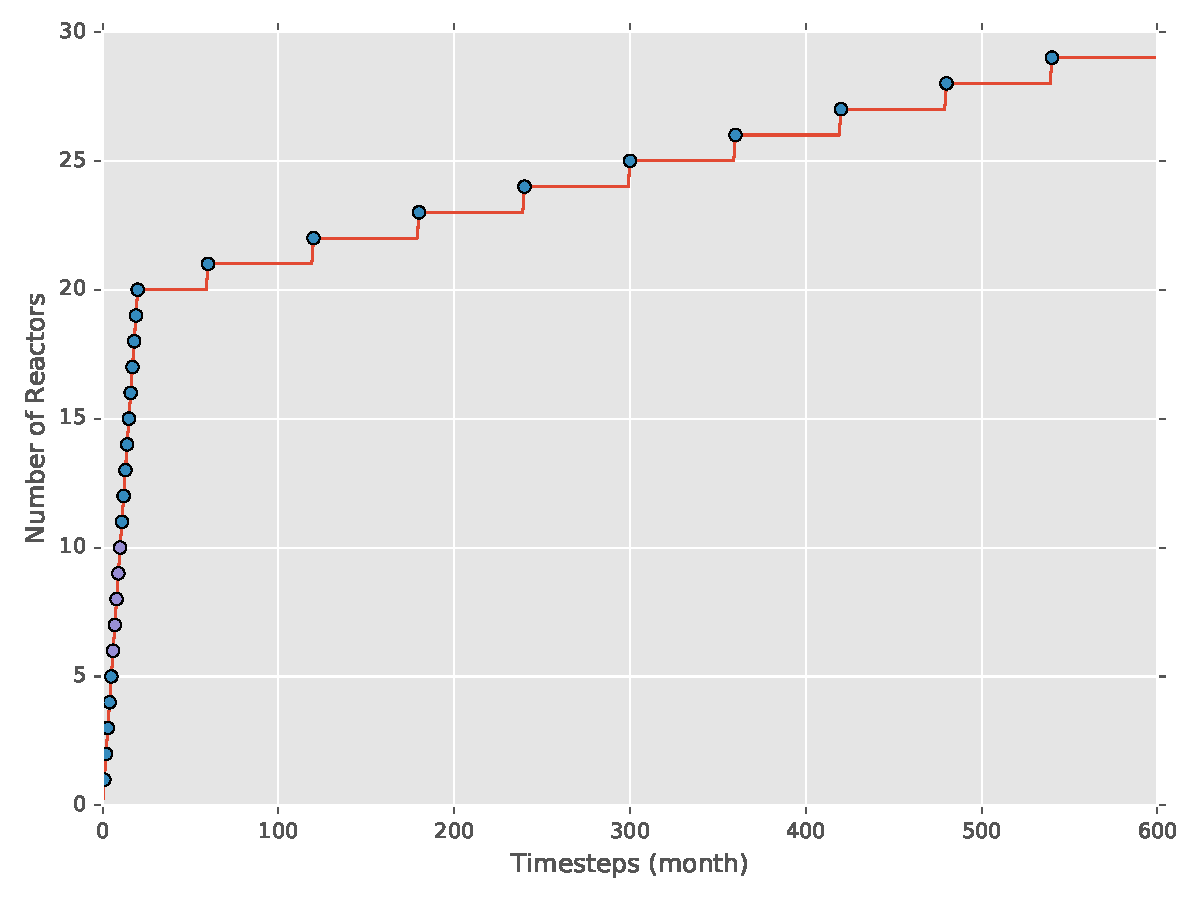
\includegraphics[width=0.75\columnwidth]{rxtr_deploy.pdf}
    \caption[]{
      \label{fig:deploy}
      Reactor deployment in each simulation as a function of simulation time
      steps. Each point in the graph is a reactor being deployed in the
      simulation. Deployments for the tariff scenario are distinguished by
      color: blue represents deployments in Region A and purple represents
      deployments in Region B.}
  \end{center}
\end{figure}

\begin{figure}
  \begin{center}
    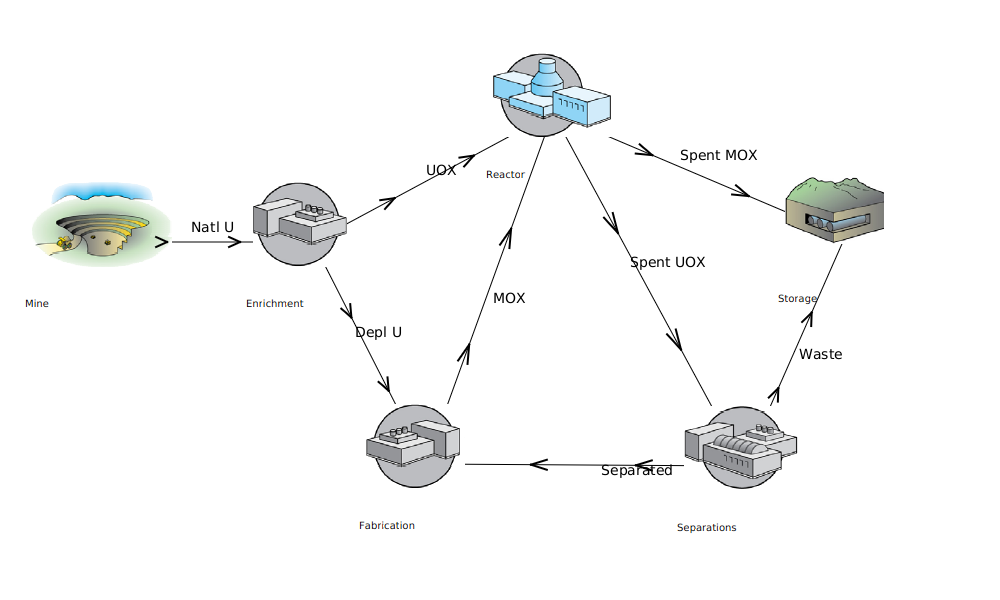
\includegraphics[width=0.75\columnwidth]{base_case_fc}
    \caption[]{
      \label{fig:base}
      Material routing between in the base case scenario, single-pass MOX fuel
      cycle. Possible arc flows are labeled with commodity names.}
  \end{center}
\end{figure}

Three perturbations from the base case scenario are used to provide examples of
modeling capability enabled through the use of the DRE. The scenarios are
summarized in Table \ref{scenarios} below and described in more detail in the
following sections. 

\begin{table}[]
\centering
\caption{Short Descriptions of Scenarios Ran}
\label{scenarios}
\begin{tabularx}{\textwidth}{|p{1.5cm}|p{1.5cm}|X|X|}
\hline
\textbf{Scenario  Name} & \textbf{Scenario Handle} & \textbf{Primary Departure from Base Case}                & \textbf{Capability Highlighted}                             \\ \hline
Separations Outage      & outage                   & Separations facility halts operation mid-simulation      & System flexibility to recycling facilities operation        \\ \hline
External MOX Supplier   & external                 & An additional supplier of MOX enters mid-simulation      & System flexibility to entry and exit of commodity suppliers \\ \hline
Regional Tariffs        & tariff                   & Two regions are modeled with dynamic trade relationships & Ability to model nontrivial international relationships     \\ \hline
\end{tabularx}
\end{table}

The first perturbation shows how the \gls{DRE} allows the system to respond to
arbitrary changes in the state of any facility.  In this case, the separations
facility shown in Figure \ref{fig:base} suffers an outage from $250 \leq t
\leq 300$, during which all other facilities continue to engage in trade,
adapting their trades for the available material.  The second perturbation
demonstrates how the \gls{DRE} can easily adapt to new facilities entering the
scenario.  An external source of MOX enters the simulation at $t = 250$ and
continues until it is exhausted.  The last perturbation demonstrates the
ability of agents to change their preference assignment algorithm dynamically
within the simulation.  In this case, it also engages the \gls{RIF} hierarchy
built into \Cyclus{} that allows for facilities to be owned by an
\textit{institution} that operates in a geopolitical \textit{region}, each of
which can influence how preferences are determined.  In this case, a second
region is added and a tariff is imposed on trade between the regions at $150
\leq t \leq 300$.

Importantly, in all cases, the only changes necessary to perturb the system
are local to the facility experiencing the perturbation.  All other
facilities, if properly configured to take advantage of flexibilities in the
base case, will automatically respond.  As such, these perturbations represent
much larger potential changes that can be introduced, either dynamically or by
user input into a fuel cycle.

A summary of the results is shown in Figures \ref{fig:uoxflow} and
\ref{fig:moxflow}.  Figure \ref{fig:moxflow} showcases the cumulative flow of
MOX fuel into all reactors as a function of simulation time step. Because
reactors can be fueled only with UOX or MOX, it represents the inverse of
Figure \ref{fig:uoxflow}. For example, whereas the tariff scenario utilizes
the most UOX, it utilizes the least MOX for the same reasons. A number of
additional features can be observed in Figure \ref{fig:moxflow} dealing with
departures from dynamic equilibrium of the base case scenario. The
undershooting and then overshooting of MOX consumption in the outage scenario
is visible. During the outage, less MOX is consumed, but immediately after the
outage, excess MOX is consumed until there is a return to dynamic
equilibrium. Additionally, a reduction in the total amount of MOX (sourced
from recycled UOX) consumed is observed in the external scenario. This is due
to a reduction in the available recycled UOX supply during periods of external
MOX consumption. In short, for each reload of external MOX, the system loses a
future amount of recyclable UOX.  A more complete discussion can be found in
Ref \citeprod{dre_paper}.

\begin{figure}
  \centering
  \begin{minipage}{\textwidth}
    \centering
    \subfloat[UOX flow.]{
      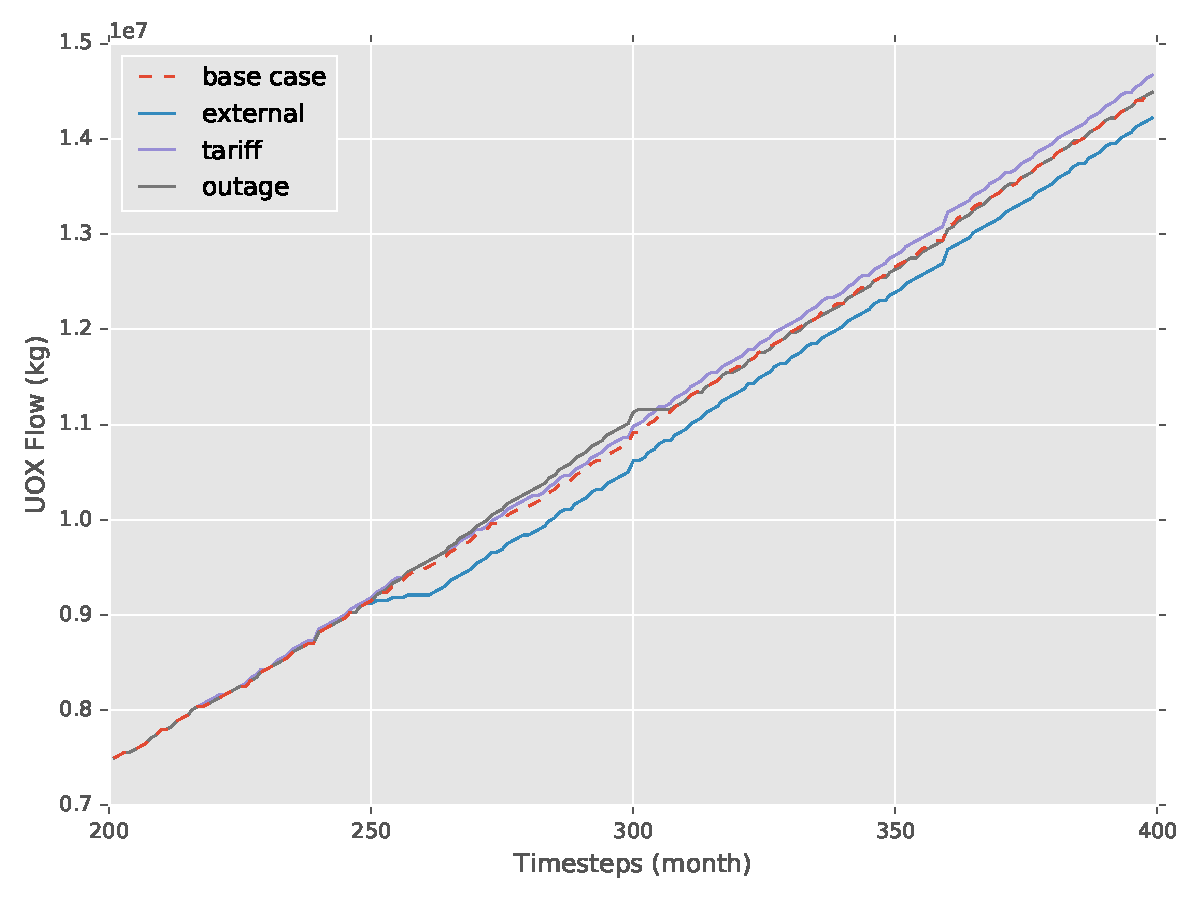
\includegraphics[width=0.5\textwidth]{uox_flow.pdf}\label{fig:uoxflow}}
    \subfloat[MOX flow]{
      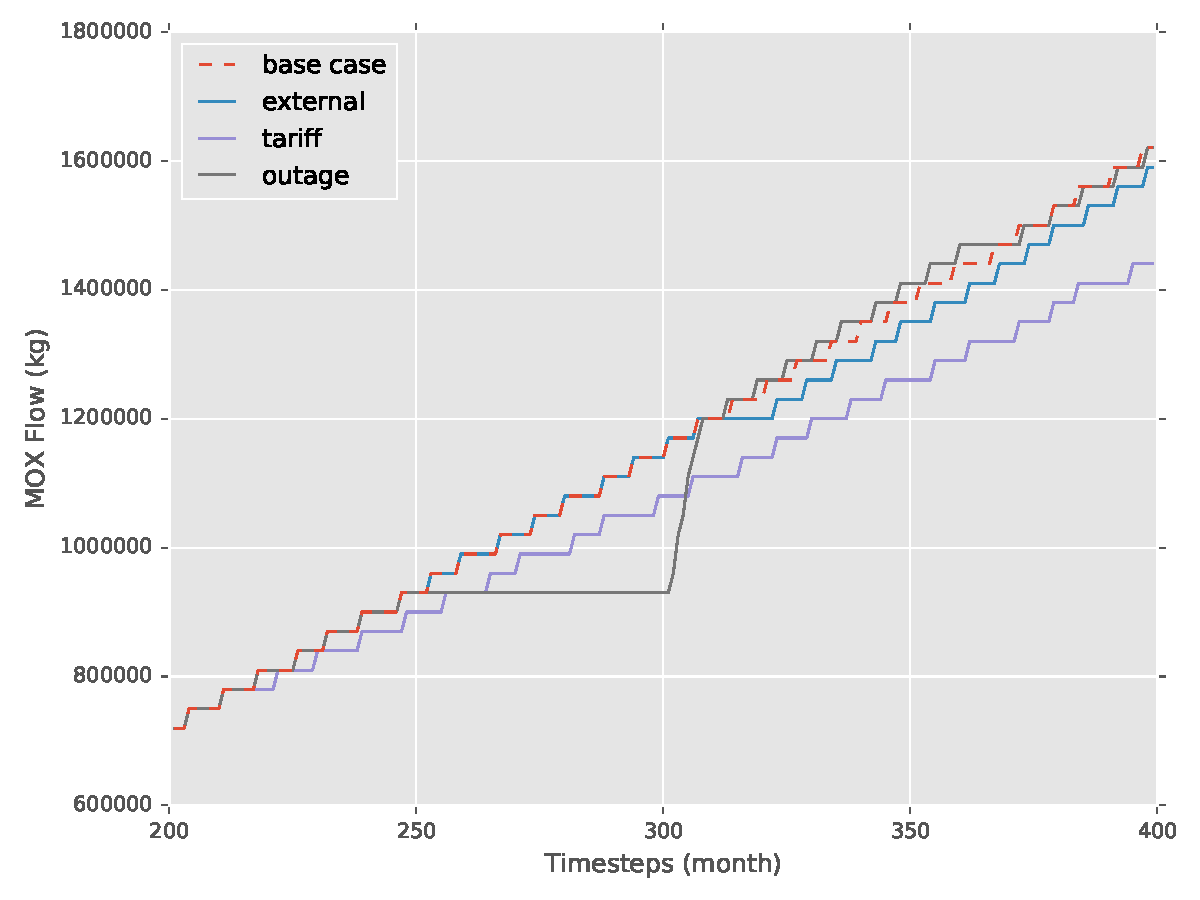
\includegraphics[width=0.5\textwidth]{mox_flow.pdf}\label{fig:moxflow}}
  \end{minipage}%
  \caption[]{
    \label{fig:flows}
    Cumulative flow of fuel in all Scenarios. The timestep period between 200
    and 400 is chosen to highlight all relevant transients. }
\end{figure}



\subsection{Objective Function Callbacks}\label{subsection:callback}

\subsubsection{Motivation}

As previously discussed, the basic implementation of the \gls{DRE} provides
the ability for consumers to evaluate different resource offers, but does not
provide the suppliers with any mechanism to judge how well those offers will
be recieved.  For suppliers that are unable to match the request exactly, but
otherwise have flexibility in the quantity and/or quality of the offers that
they issue, this leaves them essentially guessing which offers will be best
received by the consumer.  If the suppliers offers are poor matches, the
consumers may operate below their ideal performance or even experience supply
disruptions.  Three major types of remedy exist:
\begin{enumerate}
\item encourage supplier facilities to make many offers with different
  qualities/quantities,
\item increase the information included in a request to enable the supplier to
  make informed choices, or
\item provide a mechanism for the supplier to query the consumer.
\end{enumerate}

The first of these was ruled out because of the burden it would place of the
\gls{DRE} optimization algorithms.  Suppliers with continuously varying
paramter spaces might need to issue 1 or 2 orders of magnitude more offers for
each request in order to ensure that they were well-matched to the consumers
preference.  Since the performance of the \gls{DRE} scales with the number of
request-offer pairs, this would increase the time to resolve the market even
though the number of material flows wuold not change.

The second of these was ruled out because of the burden it would violate the
\Cyclus{} principle that each agent should operate as a black box to ensure
flexibility.  As each new piece of information is added to the request, all
agents would need to implement algorithms that could use that information to
guide their responses.  

This leaves the preferred solution of extending the request once to include a
function pointer that can be used by the supplier to query the consumer, in
which each consumer is free to respond to this query with as much complexity
as they require.


\subsubsection{Implementation}

Two small changes were made to give suppliers more control over the nature of
their offers and their interaction with the \gls{DRE}.  First, the contents of
a bid were expanded to include the supplier's preference for each bid.  This
information can then be used by consumers to impact their algorithm for
determining the ultimate request-bid preference.  As with the consumer's
ability to establish preference, the supplier is free to use any algorithm to
establish this preference.

The objective function callbacks have also been implemented, simply by
extending the contents of a request to include a pointer to a fcuntion with a
single argument of a single bid, and extending the interface with a function
that will return that pointer.  Suppliers are free to query the callback
function (or not) and implement any algorithm to use that information to amend
their bids.

Both of these changes require no changes to existing agent archetypes, unless
they want to take advantage of the new functionality.  A default bid
prefreence of 0 is assigned for all bids where it is not assigned explicitly,
so that all methods to generate bids will continue to function with no
changes.  Similarly, the callback functions are only queried if a supplier
archetype chooses to do so.


\subsubsection{Demonstration Problem}


This capability was demonstrated with a storage facility archetype that
determined its preference based in the specific decay heat of the offered
resource.  When added to the simulation, the archetype was configured with a
maximum specific decay heat and will never accept a material with a specific
decay heat above that threshold.  In addition, it will prefer materials with a
preference as high as possible below that threshold.

This archetype was used to fill multiple storage roles in a simulation that
also included a standard recipe reactor: wet storage with no maximum allowable
specific decay heat, dry storage with a modest maximum allowable specific
decay heat, and a geologic repository with a low maximum allowable specific
decay heat.  In such a simulation, the reactor, wet storage and dry storage
always offer their material to be taken by one of the other facilities.

There are a number of more subtle benefits of this approach.  These materials
can be offered in a single commodity market with no need to constrain the
possible flows \textit{a priori}.  If material happens to remain in wet
storage long enough that its decay heat drops sufficiently, its material can
be sent directly to the geologic repository.  All storage facilities
participate in the same market and only accept material that is suitable for
their characteristics.  In addition, intermediate storage facilities can trade
material based on its actual decay heat rather than its residence time.  Many
fuel cycle models rely on storage facilities with minimum residence times to
approximate the notion that spent-fuel transport and acceptance is typically
limited by its decay heat (among other related characteristics).  In this
case, the archetype can make decisions based on the operational characteristic
that matters rather than an approximate surrogate.

The preference function of the consumer always ensures that material only
flowed when the decay heat is sufficiently low.  In the absence of objective
function callbacks, however, the intermediate storage facilities would offer
all the resources in their inventory during every time step.  This would
result in many superfluous offers that exceeded the decay heat limits of the
consumers.  By using a callback function to probe the preference of the
receiving facility for each possible offer, it can avoid making offers that
are not going to be accepted by the receiving facility.

 
